\section{Eclipse IDE setup}
Eclipse is a popular open source Integrated Development Environment (IDE) that is widely
adopted in the developer community.

\subsection{Installing Eclipse}
\paragraph{}
Because we are both using Fedora Linux operating system, we do not require external resources to install the Eclipse IDE as it came bundled in the install DVD. Nevertheless, you need to select the following package in ordre to get it up and running:
\footnote{Some extra packages will be detected by the install system, but those listed here are the must have to compile and run this project}

\begin{enumerate}
\item eclipse-changelog
\item eclipse-jdt
\item eclipse-rcp
\item eclipse-egit
\item eclipse-pde
\item eclipse-birt
\item eclipse-dtp
\item eclipse-swt
\end{enumerate}

\paragraph{}
You can install them by using the command: \textit{\textbf{yum install [package name]}} or via the graphic interface for adding packages. In the case, you are not using Fedora or any other Linux variant you could always download the Eclipse application from the eclipse.org site. 

Exactly you need to download the \textbf{"Eclipse IDE for Java EE Developers"} available at this url:
\url{http://www.eclipse.org/downloads/packages/eclipse-ide-java-ee-developers/heliossr2}
\footnote{This URL is relative to the current version of eclipse as, so make sure to go to the correct URL if it get updated}
\footnote{This version include almost all the plugins needed to compile and run the application, we recommend you to add the git plugin to be able to download the code from GitHub}

\subsection{GlassFish plugin}
The GlassFish Tools Bundle for Eclipse is a software bundle that includes GlassFish Server v2.1
and v3 Prelude, Eclipse IDE 3.4 and the plug-in that enables them to work together. It provides
a ready-to-use environment that helps you get started with developing applications on Eclipse
and deploying them to GlassFish Server.

To Install on Linux Platform:
\begin{enumerate}
\item Go to \textbf{\textit{Help → Install}} new software 
\item Add new repository \url{http://dlc.sun.com.edgesuite.net/glassfish/eclipse/helios} to the Available software sites and name it GlassFish or any convenient name. \footnote{don't forget to change the last part of the url to your version of eclipse}
\item Select the newly created site from the "Work with" combobox. You should see them the GlassFish bundle.
\item Select the GlassFish plugin and continue to the end of the installation using next to the end.
\item Restart the IDE.
\end{enumerate}

\subsubsection{Create a new GlassFish Server}
The GlassFish Tools Bundle for Eclipse, by default, installs a new instance of GlassFish v2.1
Server and GlassFish v3 Prelude Server for you. If you want to add a new Server to Eclipse IDE, use the following procedure:

\begin{enumerate}
\item Select Servers view.
\item Select New, from Server popup menu. New Server page is displayed
\item Provide GlassFish Server details.
\item Click Next and complete Server configuration. For example, provide values for the following:
\begin{itemize}
\item Domain Directory
\item Domain Name
\item Administrator ID
\item Administrator password
\end{itemize}
\item Click Next. Add and Remove Projects page is displayed.
Select the existing projects, you want to add to the new Server.
\item Click Finish.
\end{enumerate}

\begin{figure}
  \begin{center}
  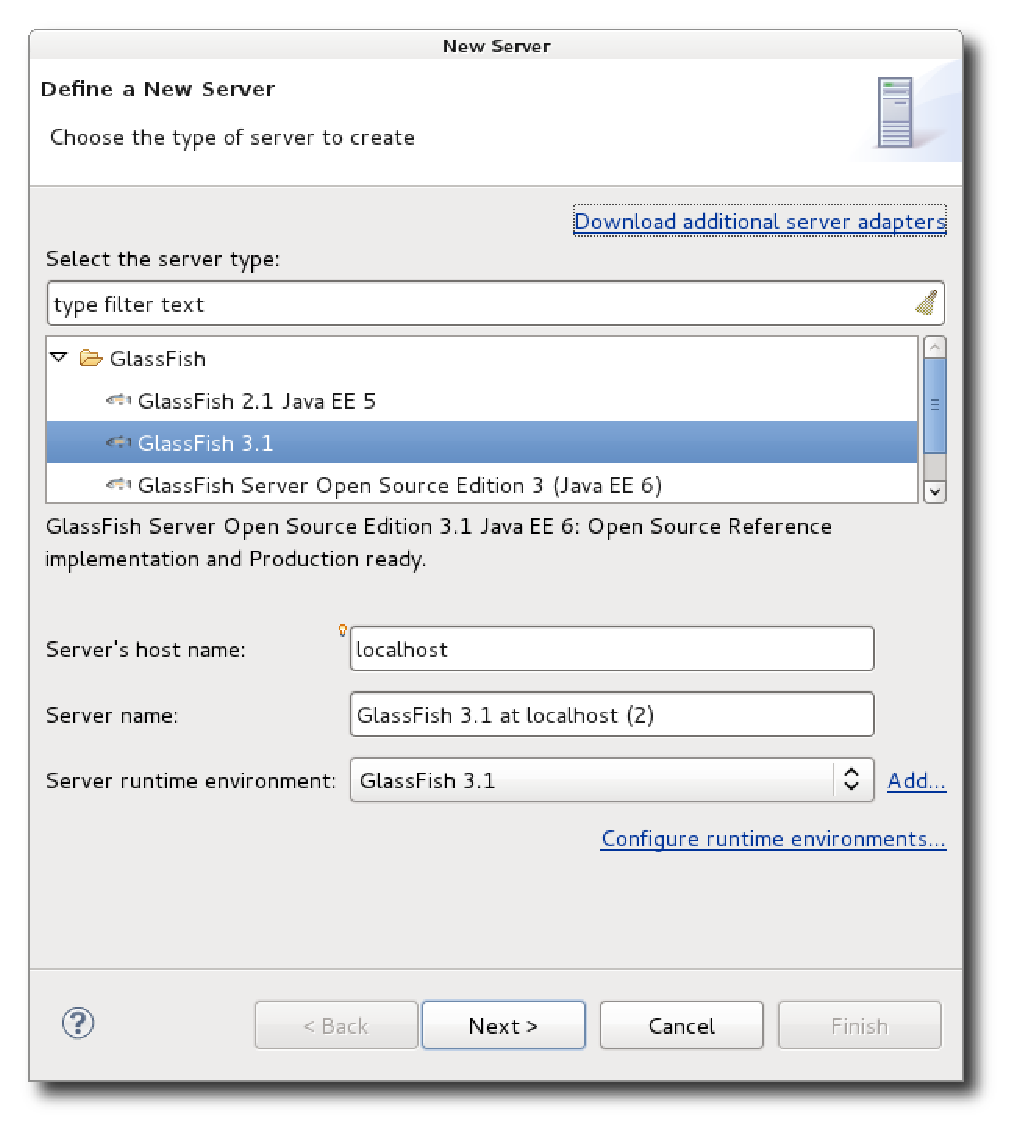
\includegraphics[scale=0.8]{Figures/Eclipse_adding_new_server.eps}
  \end{center}
  \caption{Adding new server in Eclipse}
  \label{Adding new server in Eclipse}
\end{figure}
\pagebreak

\subsubsection{To publish and clean Projects}
To publish applications to the GlassFish Server, use the following procedure:
\begin{enumerate}
\item Select Servers view.
\item Select GlassFish Server.
\item Select Publish from Server popup menu.
\end{enumerate}

To discard all published projects, and republish from scratch, use the following procedure:
\begin{enumerate}
\item Select Servers view.
\item Select GlassFish Server.
\item Select Clean... from Server popup menu.
\item Click OK to accept the warning regarding discarding the published state.
\end{enumerate}

\subsubsection{To access GlassFish Server Administration Console}
GlassFish Sever offers many administrative features that are not accessible from Eclipse IDE.
These features are available from GlassFish Server Administration Console which is accessible
from Eclipse IDE. The following procedure describes the process of accessing GlassFish Server
Administration Console, from Eclipse IDE.
\footnote{The administration console could be accessed via any navigator using the url http://localhost:4848 (assuming that your GlassFish server is installed on the local machine, you could change it to the adequate server name if accessing from an outside location)}
\begin{enumerate}
\item Select Servers view.
\item Select Server popup menu → GlassFish Enterprise Server →GlassFish Administration Console.
\end{enumerate}

\subsection{Creating the Eclipse Projects}
\subsubsection{The container project (EAR project)}
There are different Eclipse project types that can be used with the JEE 6. In the most flexible setup, you use a so-called Enterprise Application Project, also called an EAR Project, after the artifact it produces, an Enterprise Archive or EAR.

An EAR project is nothing but a container, intended to bundle the artifacts of the contained projects, along with any libraries that they use and that are not already part of the Java Enterprise Edition. We always begin with an EAR project, and then we create those projects, where we do the actual work, adding each of them to the EAR. Later, for deployment, we can export the EAR project as one single EAR file that contains all JARs from the contained projects.

In the JEE perspective you have the Project Explorer on the left side. If you have a fresh workspace, then the Project Explorer will be empty. Either from the File menu or from the Project Explorer context menu choose New / Enterprise Application Project. This opens the New EAR Application Project dialog.

\begin{figure}
  \begin{center}
  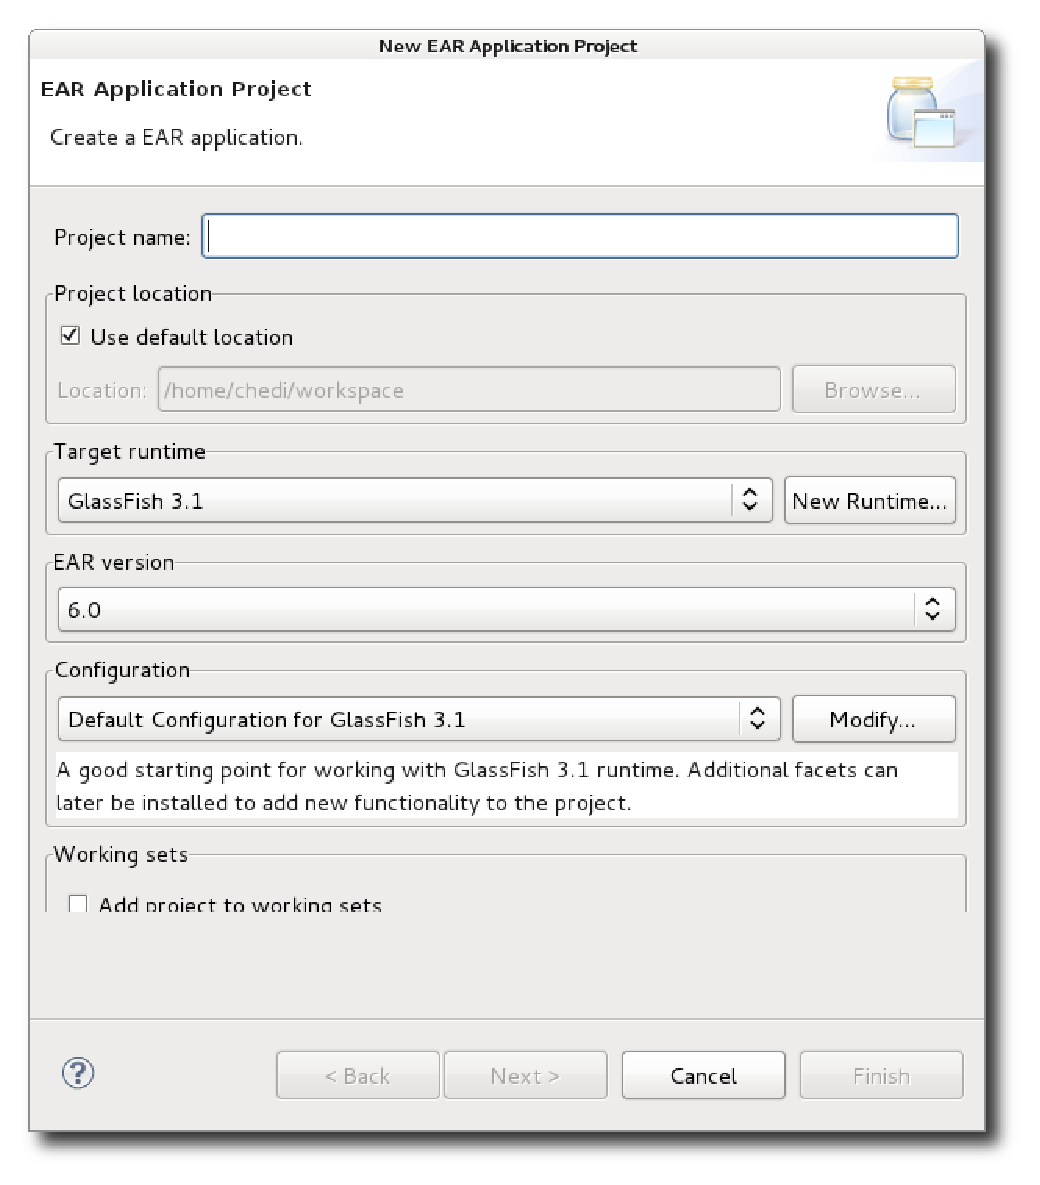
\includegraphics[scale=0.8]{Figures/New_entreprise_project_wizard.eps}
  \end{center}
  \caption{Creating Eclipse entreprise project}
  \label{Creating Eclipse entreprise project}
\end{figure}
\pagebreak

\subsubsection{The EJB project}
Enterprise Java Beans (EJB) are really just normal Java classes. It is when EJBs are instantiated under the control of an EJB container, that all sorts of interesting things begin to happen automatically.

For instance you can leave field variables in your beans uninitialized, and as long as they have the right annotations, the container injects proper instances, and for performance reasons it can do that from a pool of pre-allocated, momentarily idle instances.

One of the most important aspects of EJB containers is, that they can inject datasources (for instance JDBC datasources) and other resources, that the program only references by name, and that are really defined in the application server.

When you use JPA, an Entity is again a simple Java class with getters and setters for its fields, a POJO. You make it an entity by doing two things: annotating it with JPA annotations, and letting an EntityManager fetch it from or persist it to the database. You get such an EntityManager again via injection, when you get it, it is already associated with a persistence context that manages transactions and caches entities.